
\documentclass[11pt,a4paper]{article}
\usepackage[margin=1.7cm]{geometry}
\usepackage{amsmath,amssymb}
\usepackage{tikz}
\usepackage{xcolor}
\usepackage{parskip}
\usepackage[T1]{fontenc}
\usepackage[utf8]{inputenc}
\usepackage[dutch]{babel}
\usepackage{newtxtext,newtxmath}
\usetikzlibrary{arrows.meta,calc,positioning}

\setlength{\parskip}{0.55em}
\setlength{\parindent}{0pt}

\newcommand{\uncertain}[1]{\textit{\textcolor{gray}{#1}}}

\title{Notebook 2012 --- Pagina's 65, 66 en 69--72}
\author{}
\date{}

\begin{document}
\maketitle

\uncertain{Pagina's 67 en 68 zijn op verzoek overgeslagen. Deze batch bevat vooral formulebladen, korte definities en een Doppler-afleiding. Minder scherpe symbolen zijn zo letterlijk mogelijk overgenomen en als onzeker gemarkeerd waar nodig.}

\clearpage
\section*{Pagina 65}

\begin{minipage}[t]{0.48\textwidth}
\subsection*{Linkerhelft}

Frequentie van een object wordt\\
$20\%$ hoger voor een observator.

\begin{center}
\begin{tikzpicture}[>=Latex,scale=0.9]
    \fill (0,0) circle (0.05);
    \draw[->] (-2,0) -- (-0.35,0) node[midway,above] {$v_s$};
    \draw[->] (0.35,0) -- (2.0,0) node[midway,above] {$v$};
\end{tikzpicture}
\end{center}

\begin{align*}
N_1 &= \left(\frac{V}{V-v_s}\right)N 
\qquad \text{= op je af}
\\[0.3em]
N_1 &= \left(\frac{V}{V+v_s}\right)N
\qquad \text{= van je af}
\end{align*}

\begin{align*}
N_1 &= \left(\frac{V}{V-v_s}\right)n
\\
\frac{V-v_s}{V} &= \frac{n}{n_1}
= \frac{100\%}{120\%}
= \frac{5}{6}
\\
1-\left(\frac{v_s}{V}\right) &= \frac{5}{6}
\\
\frac{v_s}{V} &= 1-\frac{5}{6} = \frac{1}{6}
\end{align*}

\begin{align*}
\frac{V+v_s}{V} &= \frac{n}{n_2}
\\
1+\left(\frac{v_s}{V}\right) &= \frac{n}{n_2}
\\
1+\frac{1}{6} &= \frac{n}{n_2}
\\
\frac{7}{6} &= \frac{n}{n_2}
\\
n_2 &= \frac{6}{7}n
\end{align*}

\[
\frac{n-n_2}{n}\times 100
=
\left(1-\frac{6}{7}\right)\times 100
\approx 16{,}7\%
\]
\end{minipage}
\hfill
\begin{minipage}[t]{0.48\textwidth}
\subsection*{Rechterhelft}

\[
700\ \text{Hz}
\]

\begin{center}
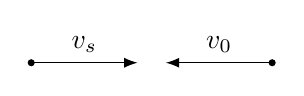
\begin{tikzpicture}[>=Latex,scale=0.9]
    \fill (-1.7,0) circle (0.05);
    \fill (1.7,0) circle (0.05);
    \draw[->] (-1.7,0) -- (-0.2,0) node[midway,above] {$v_s$};
    \draw[->] (1.7,0) -- (0.2,0) node[midway,above] {$v_0$};
\end{tikzpicture}
\end{center}

\[
N_1 = \left(\frac{V+v_0}{V-v_s}\right)N
\]

\[
\text{Hoekmoment} = mVR
\]
\end{minipage}

\clearpage
\section*{Pagina 66}

\begin{minipage}[t]{0.48\textwidth}
\subsection*{Linkerhelft}

\begin{align*}
R_\infty
&=
\frac{\alpha^2 m_e c}{4\pi \hbar}
=
\frac{\alpha^2}{2\lambda_e}
=
\frac{\alpha}{4\pi a_0}
\\[0.5em]
hcR_\infty
&=
m_e c^2\frac{\alpha^2}{2}
=
\frac{hc\,\alpha^2}{2\lambda_e}
=
\frac{h f_c \alpha^2}{2}
\\[0.5em]
\frac{\hbar\omega_c}{2}\alpha^2
&=
\frac{\hbar^2}{2m_e a_0^2}
=
\frac{e^2}{(4\pi\varepsilon_0)\,2a_0}
\end{align*}

\uncertain{De eerste noemer is geschreven als $4\pi\hbar$, wat equivalent is aan $2h$.}
\end{minipage}
\hfill
\begin{minipage}[t]{0.48\textwidth}
\subsection*{Rechterhelft}

\begin{align*}
\lambda_e &= \text{Compton golflengte}
= \frac{h}{m_e c}
\\[0.4em]
f_c &= \text{Compton frequentie}
= \frac{m_e c^2}{h}
\\[0.4em]
\omega_c &= \text{Compton moment}
= 2\pi f_c
\end{align*}
\end{minipage}

\clearpage
\section*{Pagina 69}

\begin{minipage}[t]{0.46\textwidth}
\subsection*{Linkerhelft}

Bron:

minim JavaScript

Daniel Tammet $\rightarrow$ hoofd rekenen
\end{minipage}
\hfill
\begin{minipage}[t]{0.50\textwidth}
\subsection*{Rechterhelft}

Snelheid van fonon

\begin{align*}
V &= f \times \lambda
\\
f &= \frac{1}{2\pi}\omega
\\
f &= \frac{1}{2\pi}\sqrt{\frac{K}{m}}
\\[0.5em]
V &= \frac{1}{2\pi}\sqrt{\frac{K}{m}}\;\lambda
\\
V &= \frac{1}{2\pi}\sqrt{\frac{F_{\max}}{2R_p m_p}}\,(2R_c)
\\
V &= \left(\frac{R_c}{\pi}\right)\sqrt{\frac{F_{\max}}{2R_p m_p}}
\end{align*}
\end{minipage}

\clearpage
\section*{Pagina 70}

\begin{minipage}[t]{0.48\textwidth}
\subsection*{Linkerhelft}

\[
E = h f
\]

\begin{align*}
C_e &= f\lambda
\\
c &= \frac{\varepsilon_0 A}{D}
\\
E &= \frac{Q^2}{2C}
\end{align*}

fotoElektrisch effect

\begin{align*}
(1)\quad C_e &= f\lambda
\quad \Rightarrow \quad
\lambda = \frac{C_e}{f}
\\[0.3em]
(2)\quad c &= \frac{\varepsilon_0 A}{D}
\quad \Rightarrow \quad
c = \frac{\varepsilon_0 \lambda^2}{0.5\,\lambda}
\\[0.3em]
(3)\quad c &= \frac{\varepsilon_0 \lambda^2}{0.5\,\lambda}
\quad \Rightarrow \quad
c = 2\varepsilon_0\lambda
\\[0.3em]
(4)\quad c &= 2\varepsilon_0\lambda
\quad \Rightarrow \quad
c = \frac{2\varepsilon_0 C_e}{f}
\\[0.3em]
(5)\quad E &= \frac{Q^2}{2C}
\quad \Rightarrow \quad
E = \frac{Q^2 f}{4\varepsilon_0 C_e}
\end{align*}

\[
\varepsilon_0
=
\text{max amplitude van het di\"elektrum}
\]
\[
\text{hier van het vacu\"um (tijdruimte)}
\]
\end{minipage}
\hfill
\begin{minipage}[t]{0.48\textwidth}
\subsection*{Rechterhelft}

\[
f_c = \frac{m_e c^2}{h}
\qquad
\omega_c = 2\pi f_c
\]

\[
V = \omega_e R_c
\qquad
\omega_e = \sqrt{\frac{K_e}{m_e}}
\qquad
K_e = \frac{F_{\max}}{R_x}
\]

\textbf{Vrije vortex}

\begin{align*}
C_e &= C_i\,R_e\,N
\\
C_e &= \sqrt{\frac{K_e}{m_e Z}}\;R_c\,N
\\
C_e &= \sqrt{\frac{F_{\max}}{R_x m_e Z}}\;R_c\,N
\\
C_e^2 &= \frac{F_{\max}}{R_x m_e Z}\;R_c^2 N^2
\\[0.4em]
R_x &= N^2
\left[
\frac{F_{\max} R_c^2}{m_e C_e^2 Z}
\right]
\end{align*}

Basis formules

\medskip

elektronen Radius
\end{minipage}

\clearpage
\section*{Pagina 71}

\begin{minipage}[t]{0.48\textwidth}
\subsection*{Linkerhelft}

\begin{align*}
a_0 &= \frac{F_{\max} R_c^2}{m_e C_e^2}
\\[0.4em]
a_0 &= h\cdot \frac{c^2}{8\pi F_{\max} C_e R_c}
\\[0.4em]
a_0 &= \frac{c^2 R_c}{2C_e^2}
\\[0.4em]
\frac{1}{R_c} &= \frac{c^2}{a_0\,2C_e^2}
\\[0.4em]
a_0 &= \frac{h}{4\pi m_e C_e}
\\[0.4em]
h &= 4\pi m_e C_e a_0
\\[0.4em]
h &= \frac{4\pi F_{\max} R_c^2}{C_e}
\\[0.4em]
\alpha &= \frac{2C_e}{c}
\\[0.4em]
m_e &= \frac{2F_{\max} R_c}{c^2}
\end{align*}
\end{minipage}
\hfill
\begin{minipage}[t]{0.48\textwidth}
\subsection*{Rechterhelft}

\begin{align*}
R_x &= n^2
\left(
\frac{F_{\max} R_c^2}{m C_e^2 Z}
\right)
\\[0.5em]
R_\infty &= \frac{m_e c \alpha^2}{2h}
\\[0.5em]
\frac{C_e e^2}{8\pi\varepsilon_0 R_c^2 c F_{\max}}
&= \alpha
\\[0.5em]
R_e &= 2R_c
\\
R_e &= \frac{e^2}{4\pi\varepsilon_0 m_e c^2}
\\[0.5em]
a_0 &= \frac{\alpha}{4\pi R_\infty}
\\[0.5em]
\alpha_g &= \frac{Gm_e^2}{\hbar c}
= \left(\frac{m_e}{m_{\text{planck}}}\right)^2
= (t_p f_c)^2
\\[0.5em]
e &= \sqrt{2\alpha h \sqrt{\mu_0 c_0}}
\end{align*}

\[
\text{Hoekmoment} = mv_e
\]
\end{minipage}

\clearpage
\section*{Pagina 72}

\begin{minipage}[t]{0.48\textwidth}
\subsection*{Linkerhelft}

Formules

\begin{align*}
E &= mc^2\left(\frac{1}{\sqrt{1-v^2/c^2}}-1\right)
\\
E &= h f
\\
E &= \frac{1}{2}Kx^2
\\
E &= \frac{2q^2}{4\pi\varepsilon_0}\cdot \frac{1}{x}
\\[0.4em]
\omega &= \sqrt{\frac{K}{m}}
\\
\omega &= 2\pi f
\\
f &= \frac{1}{2\pi}\omega
\\
V &= f\lambda
\\
K &= \frac{F_{\max}}{x}
\\
K &= \frac{2\pi}{\lambda}
\\
\lambda &= \frac{h}{mc}
\\
\lambda &= \frac{h}{p}
\end{align*}

\begin{align*}
C_e &= \frac{c\alpha}{2}
\\
C_e &= \omega R_c
\\
a_0 &= \frac{c^2R_c}{2C_e^2}
\\
a_0 &= \frac{F_{\max}R_c^2}{m_e C_e^2}
\\
a_0 &= \frac{4\pi\varepsilon_0\hbar^2}{m_e e^2}
\\
a_0 &= \frac{\hbar}{m_e c\alpha}
\\
E &= \frac{1}{2}mv^2
\\
W &= \vec{F}\cdot\vec{x}
\\
F &= ma
\\
a &= \frac{v}{t}
\\
v &= \frac{s}{t}
\end{align*}
\end{minipage}
\hfill
\begin{minipage}[t]{0.48\textwidth}
\subsection*{Rechterhelft}

\[
\omega = mg
\]

\begin{align*}
x' &= \frac{x-vt}{\sqrt{1-v^2/c^2}}
\\[0.4em]
t' &= \frac{t-\dfrac{v}{c^2}x}{\sqrt{1-v^2/c^2}}
\\[0.6em]
\lambda_e &= \frac{h}{m_e c}
\\
f_c &= \frac{m_e c^2}{h}
\\
\omega_c &= 2\pi f_c
\\[0.6em]
E_e &= \frac{4\pi F_{\max} R_c^2}{C_e}\cdot f_e
\\[0.6em]
a &= -\omega^2 x
\\
a &= -4\pi^2 f^2 x
\end{align*}
\end{minipage}

\end{document}
